\documentclass{scrreport}
\usepackage[utf8]{inputenc}
\usepackage{float}
\usepackage{graphicx} 

% Add any additional packages you may need here

\renewcommand*{\thesection}{\Roman{section}}
\renewcommand*{\thesubsection}{\arabic{subsection}}
\renewcommand*{\thesubsubsection}{\roman{subsubsection}}

\title{Milestone Report}
\subtitle{Open Source Integration of Hummingbot with Cardano}

\author{Gen-X Degens}
\date{July 25th, 2024}

\begin{document}

\maketitle

\section{Introduction}

Decentralized exchanges (DEXs) have become a foundational component of every \
Decentralized Finance (DeFi) ecosystem. By enabling peer-to-peer trading without the \
need for intermediaries, DEXs uphold the core principles of decentralization and \
autonomy that are central to the blockchain ethos. DEXs facilitate direct transactions \
between users through smart contracts, ensuring transparency and security.

There are two primary types of DEXs: Automated Market Makers (AMMs) and order book-based \
DEXs. AMMs, such as Uniswap and Balancer, rely on liquidity pools where users can trade \
against the pool's assets using predefined algorithms to determine prices. This model \
offers continuous liquidity and is generally easier to use. On the other hand, order \
book-based DEXs, like Genius Yields and MuesliSwap, operate similarly to traditional exchanges, where buy \
and sell orders are matched directly between users. This model is favored by traders \
seeking more control over their transactions and pricing.

The dynamic nature of DEXs makes them a fertile ground for continued innovation. New \
mechanisms for liquidity provision, improved user interfaces, and enhanced security \
features are continually being developed, driving the evolution of the DeFi landscape.
\newline

Hummingbot is an open-source algorithmic trading platform designed to provide traders \
with a comprehensive toolkit to automate their trading strategies across multiple \
centralized and decentralized cryptocurrency exchanges. Developed in Python, Hummingbot \
offers a flexible and customizable framework for traders to efficiently implement, \
deploy, and execute various algorithmic trading strategies, including sophisticated \
market making, arbitrage, and directional strategies.

One of the key features of Hummingbot is its abstraction of exchange and blockchain APIs, \
which allows for the portability of trading strategies across venues. Traders can deploy \
their strategies across various exchanges simultaneously, thus maximizing their \
opportunities.
\newline

The project aims to integrate Hummingbot with decentralized exchanges (DEXs) on the \
Cardano blockchain. By enabling the users of Hummingbot to deploy their strategies, we \
seek to enhance liquidity and trading efficiency within the Cardano DEX ecosystem, \
ultimately contributing to the growth and development of decentralized finance (DeFi) on \
the Cardano platform.

This milestone report will provide an overview of the Cardano DEX ecosystem and describe \
the selection criteria leading to the identification of two implementation targets. \
Finally, we will provide a concrete implementation plan for the selected targets.

\section{The Cardano DEX Ecosystem}

The Cardano blockchain has experienced notable growth in its decentralized exchange \
(DEX) ecosystem following the integration of smart contract capabilities, a development \
marked by the Alonzo upgrade. This upgrade facilitated the execution of Plutus scripts, \
catalyzing the emergence of the first Cardano-based DEXs.

Cardano employs a distinct Extended Unspent Transaction Output (EUTxO) model, setting it \
apart from the account-based model utilized by Ethereum's EVM. In contrast to the EVM’s \
model where the state is mutable and continuously updated, the EUTxO model treats each \
transaction as a discrete state. This approach enhances security by enabling transactions \
to be processed concurrently, which reduces bottlenecks and mitigates common exploits \
found in account models. This architectural difference profoundly influences the design \
and functionality of DEXs on Cardano, necessitating that developers adapt their interfaces \
and transaction logic to exploit the strengths and address the limitations of the EUTxO model. \
It is worth mentioning that the EUTxO model also poses some chalanges, although meny teams set out \
to build a perpetual DEX on cardano, we were unable to find a functioning perpetual DEX, with all teams citing \
the difficulty of developing such instruments on top of the EUTxO. 

The Cardano DEX landscape features several prominent platforms, each contributing uniquely \
to the ecosystem’s liquidity and functionality:

\begin{itemize}
  \item \textbf{Minswap}: A versatile multi-pool DEX offering liquidity mining, yield farming, \
  and support for multiple liquidity pools for the same token pair, enhancing transaction \
  efficiency and reducing slippage.
  \item \textbf{SundaeSwap}: A user-friendly DEX with a focus on security and privacy, \
  offering a wide range of trading pairs and competitive fees to attract a diverse user base.
  \item \textbf{MuesliSwap}: Distinguished by its innovative order book model, a rarity among \
  DEXs that typically rely on automated market makers (AMMs), facilitating traditional \
  trading strategies within a decentralized context.
  \item \textbf{DEXHunter}: Focuses on user-friendly interface and hardware wallet integration, \
  appealing to both novice and seasoned traders prioritizing security and ease of use.
  \item \textbf{AXO}: A newer entrant emphasizing cross-chain interoperability and reduced \
  transaction fees, aimed at attracting a broader user base seeking economical trading options.
  \item \textbf{Blueshift}: Offers curated investment portfolios, or "oracles," which dynamically \
  adjust asset allocations based on predefined strategies to optimize returns.
  \item \textbf{Genius Yields}: A relatively new order book DEX that leverages the EUTxO model \
  to enable complex trading strategies, such as limit orders and stop-loss orders, within a \
  decentralized framework.
\end{itemize}

Each platform enhances the vibrancy and dynamic evolution of the Cardano DeFi market.
\begin{figure}[H]
  \centering
  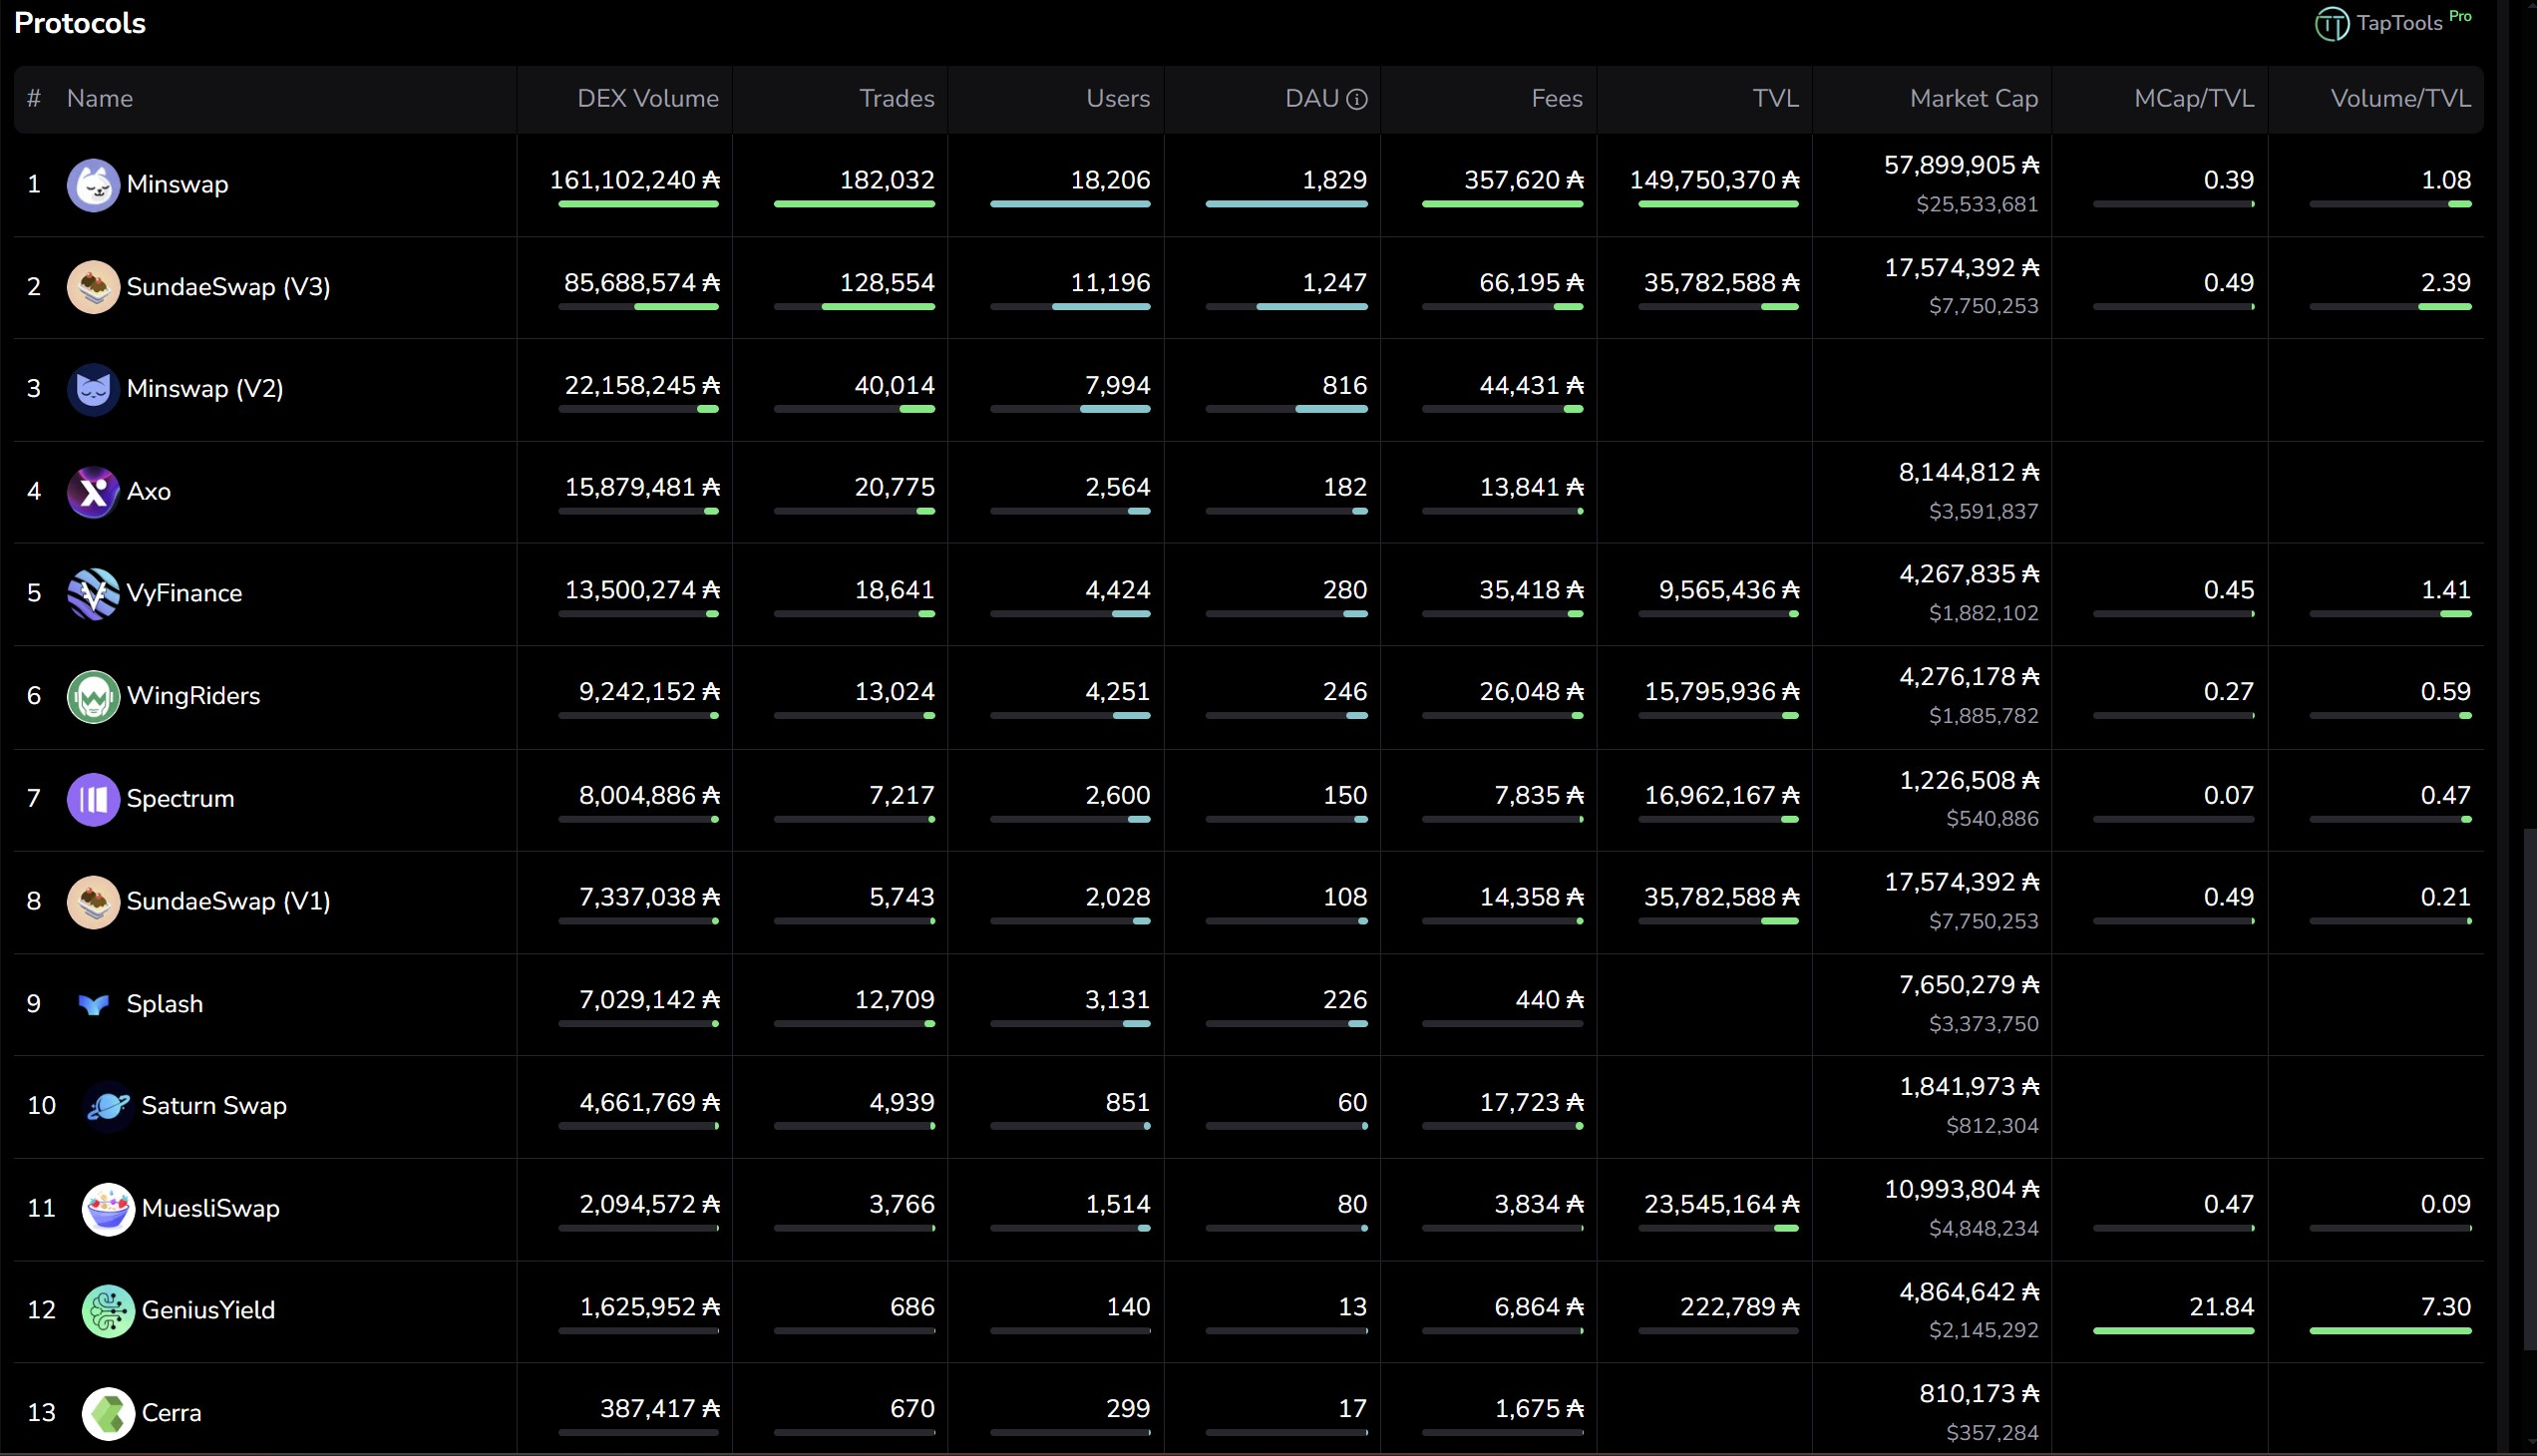
\includegraphics[width=\textwidth]{CardanoDEXs - List.jpg}
  \caption{Overview of major DEXs on Cardano}
  \label{fig:cardano_dex}
\end{figure}

\begin{figure}[H]
  \centering
  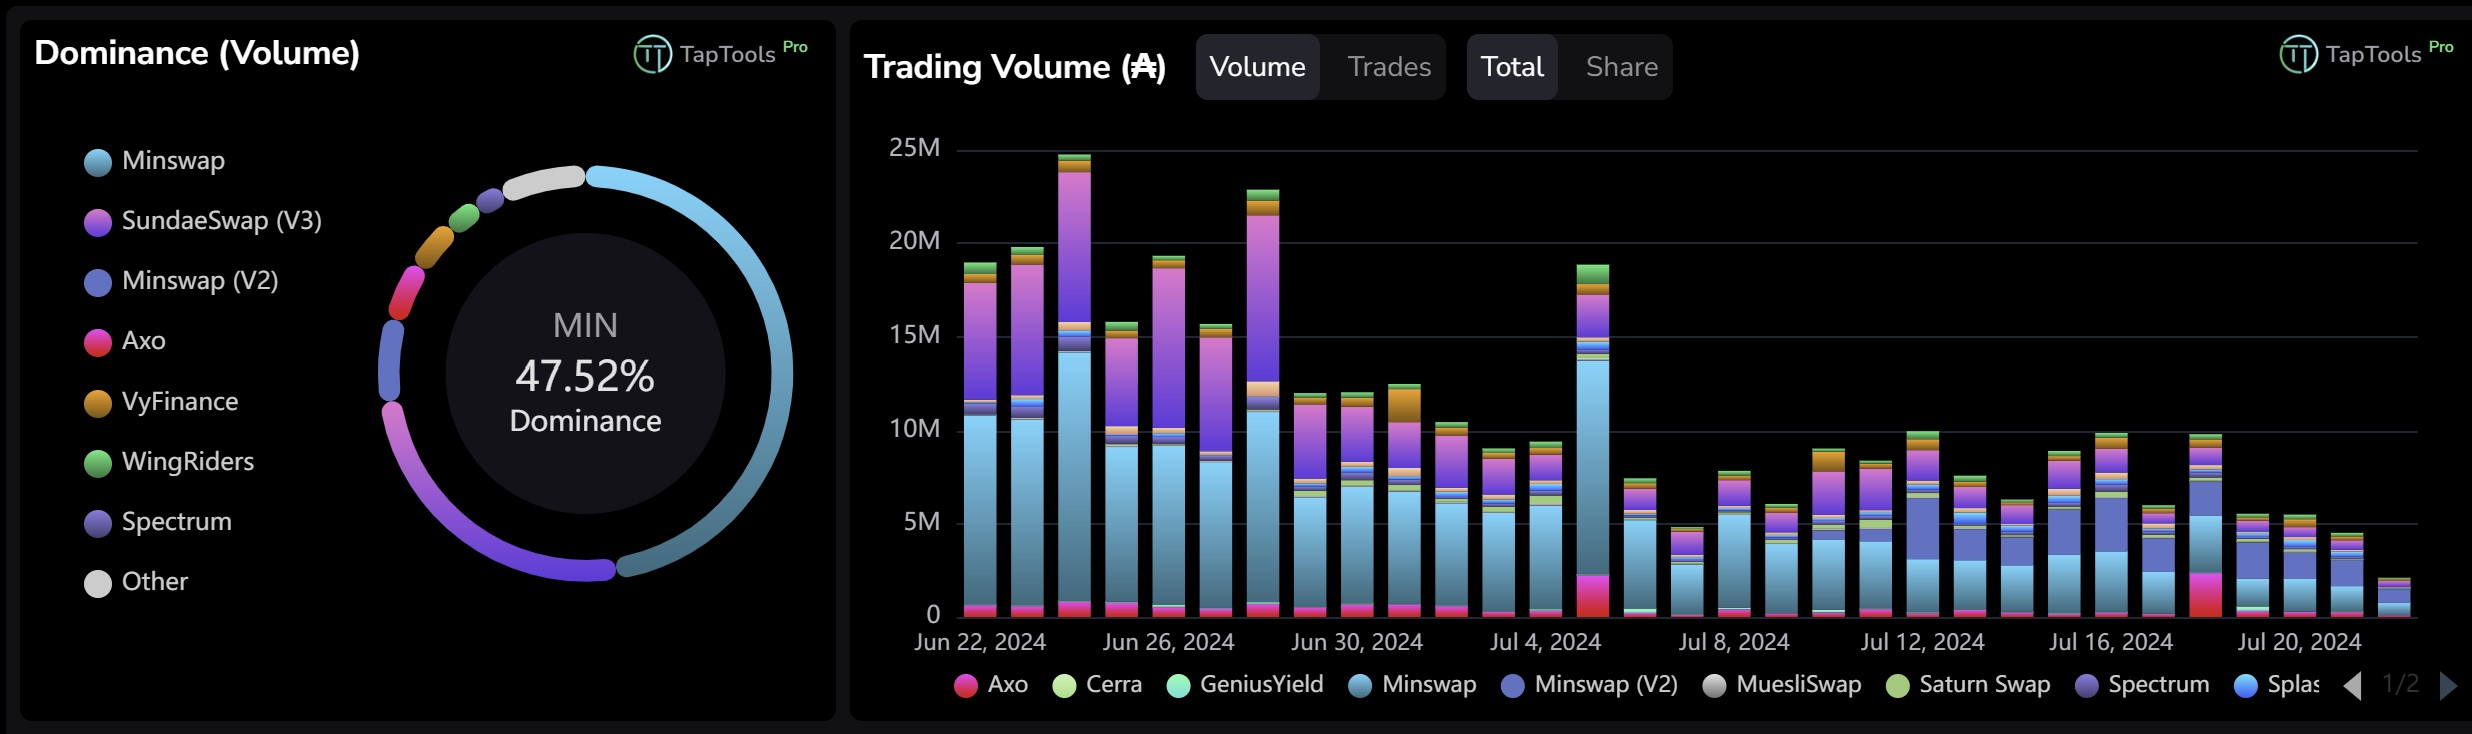
\includegraphics[width=\textwidth]{CardanoDEXs - Volume.jpg}
  \caption{Trading volume of major DEXs on Cardano}
  \label{fig:cardano_dex}
\end{figure}


\begin{figure}[H]
  \centering
  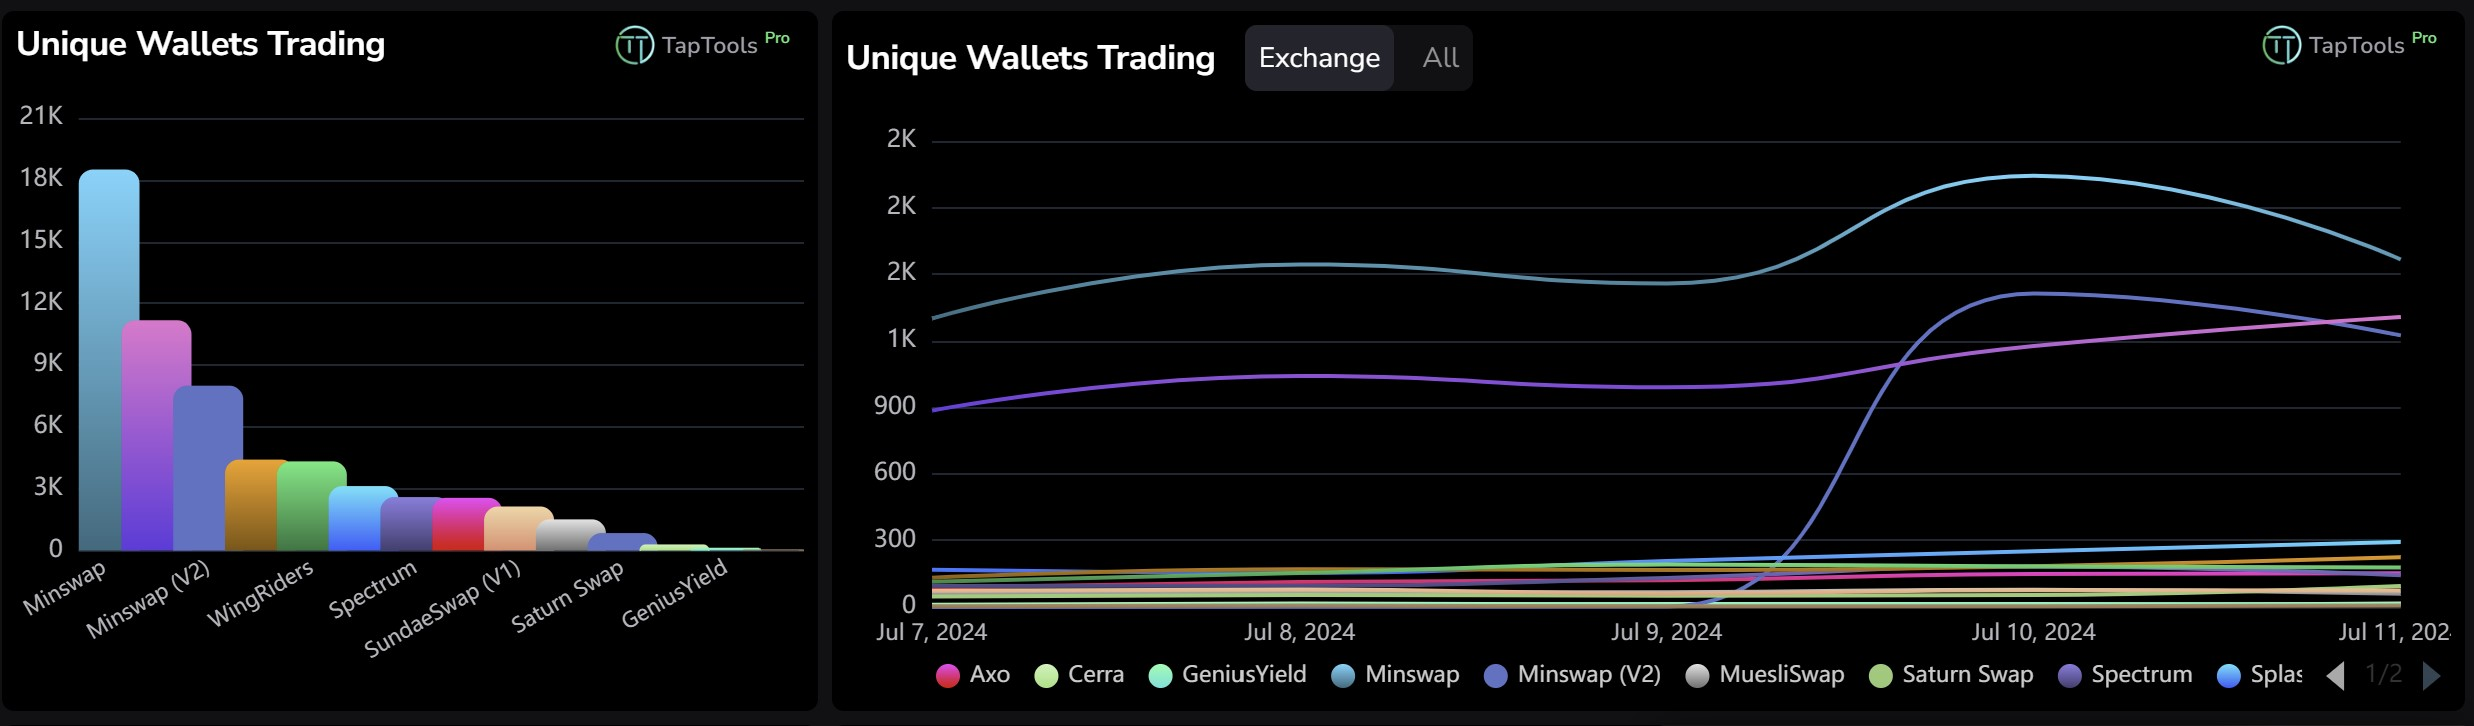
\includegraphics[width=\textwidth]{CardanoDEXs - Wallets.jpg}
  \caption{Active wallets on major DEXs on Cardano}
  \label{fig:cardano_dex}
\end{figure}

While the Cardano DEX ecosystem is still in its nascent stages, the rapid growth and continuous innovation is apparent.
The figures above provide an overview of the major DEXs on Cardano, highlighting the trading volume and active wallets on each platform.


  \section{Selection Criteria for Implementing Connectors in Cardano Decentralized Exchanges}

  When evaluating decentralized exchanges (DEXs) on the Cardano blockchain for 
  implementing connectors, it is essential to focus on three critical aspects: 
  relevance, feasibility, and impact. These criteria ensure that the selected 
  connectors not only align with the current needs and future potential of the 
  Cardano ecosystem but also can be realistically implemented and deliver 
  substantial benefits.
  
  \subsection{Relevance}
  
  \textbf{Relevance} refers to the extent to which a DEX is already adopted or 
  meets the needs of its users and the broader Cardano community. This involves evaluating the current user
  base and adoption rate of the DEX within the Cardano ecosystem, considering metrics such 
  as the number of active users, Total Value Locked (TVL) and transaction volume.
  
  \subsection{Feasibility}
  
  \textbf{Feasibility} focuses on the technical practicality and likelihood of 
  successfully implementing a hummingbot conetor for a given DEX. This involves evaluating the availability and 
  maturity of Application Programming Interfaces (APIs) and Software 
  Development Kits (SDKs) that facilitate the developement of connectors. 
  Mature and well-documented APIs and SDKs significantly enhance the 
  feasibility of implementation. 
  
  \subsection{Impact}
  
  \textbf{Impact} refers to the potential effects of implementing a connector
  for the DEX on the exchange and the broader Cardano ecosystem. 
  This includes assessing the potential of the connectors 
  to enhance market liquidity for Cardano native tokens, facilitating 
  smoother and more efficient trading experiences for users, and serving as an example for future connectors to be developed.


  \section{Conclusion}
  
  After careful consideration in accordance selection criteria, we have selected to implement connectors 
  for Minswap (https://minswap.org/) and SundaeSwap (https://app.sundae.fi/). Minswap and SundaeSwap are both 
  decentralized exchanges (DEXs) built on the Cardano blockchain. Minswap is the most used DeFi app on Cardano, 
  while SundaeSwap is an automated market maker DEX with a strong community. Each comes with their own native 
  token MIN and SUNDAE respectively.

  These two protools are highly relevant as they are and have been the most liquid and most widely used among 
  the Cardano dexes. This can be seen across different metrics such as total number of unique wallets, but also 
  on the TVL and maybe more importantly on the volume traded (according to DefiLlama). We expect that focusing 
  on the largest and most popular Dexes will have maximum impact by making trading via hummingbot available. 
  In terms of feasibility, both are mature project with fairly well developed APIs that can be leveraged. 
  It is expected that the integration work will be in the form of using the APIs rather than extending them.
  
  From a technical perspective both protocols can be accessed via popular API services. In this case, for 
  Minswap one can use Blockfrost while for SundaeSwap, Maesto.

\section{Project Plan}

The Gantt chart below outlines the project plan for the integration of Hummingbot with Minswap and SundaeSwap. 
Note that the project has been delayed due to the need to approve a change in scope. we have startes imlementation and will employ additional resources to ensure timely delivery.

\begin{figure}[H]
  \centering
  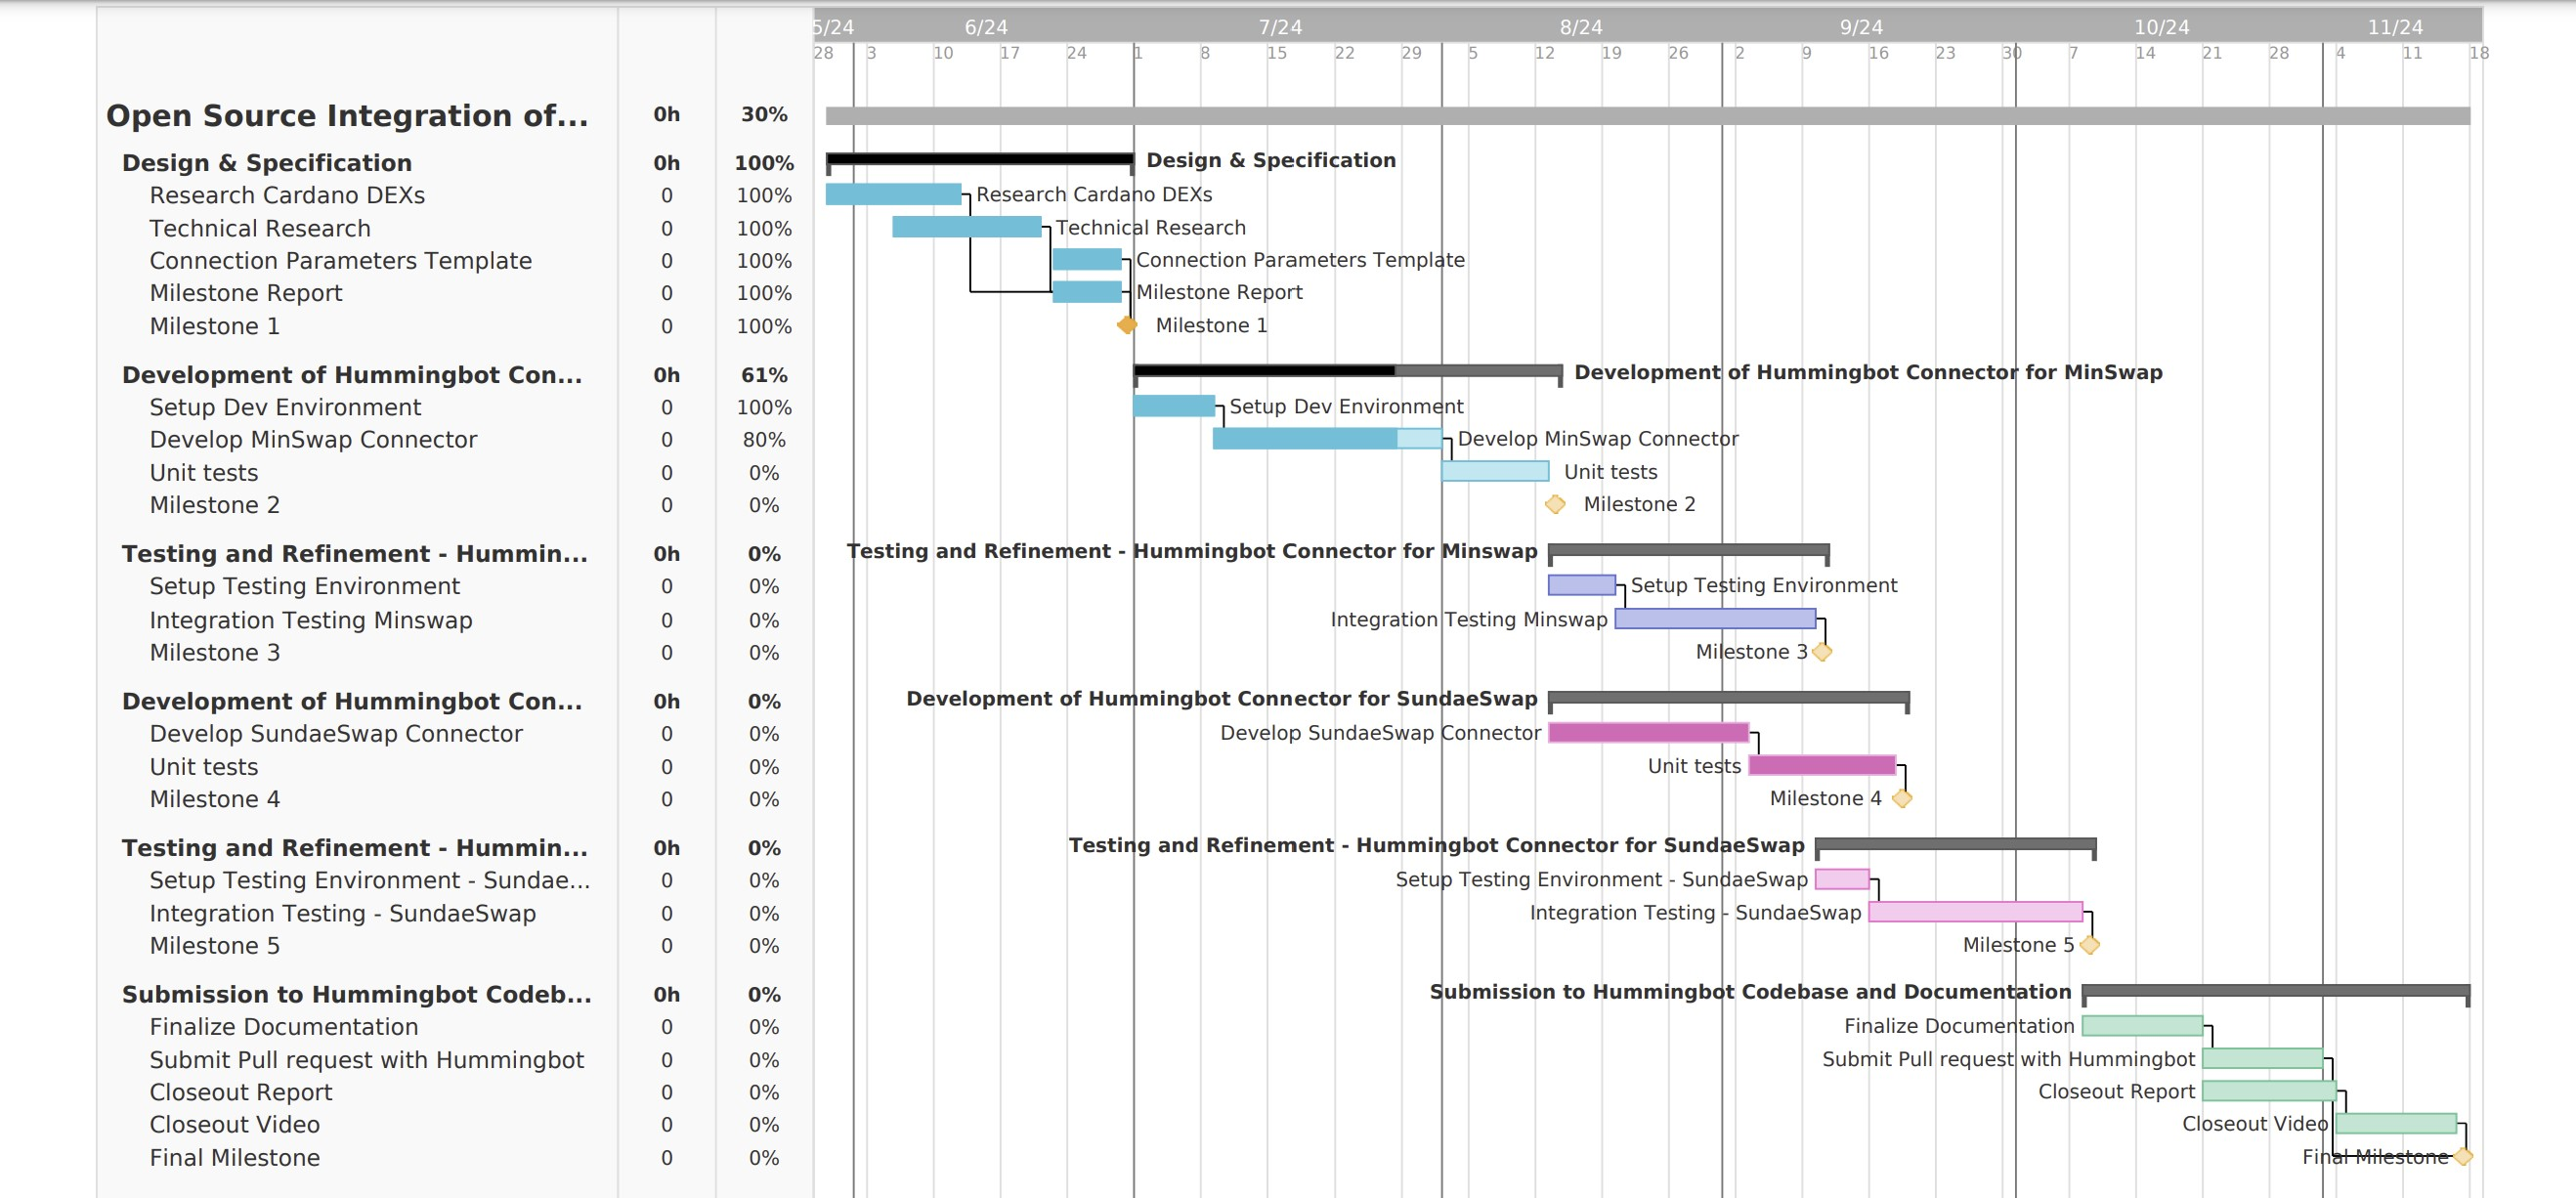
\includegraphics[width=\textwidth]{Project plan.jpg}
  \caption{Project Plan}
  \label{fig:cardano_dex}
\end{figure}



\end{document}
